% Clerics vs militias vs raduds
% use public spphere in this chapter,
"This looks like Las Vegas now," a friend mentioned to me while we walked down Qibla street. It's a few days before Ashura in August 2021, and a blisteringly hot 45°C weather in August 2021. The streets are filled with hungry and thirsty pilgrims, many of whom have traveled multiple days by foot or vehicle for Ashura. 

Finding it hard to disagree with my friend, I looked around at the variety of service tents, known as \emph{mūkib}\footnote{See chapter \ref{chapter-2} for an expanded explanation on the institution of \emph{muwālkib} and their role in Karbalaei history.}, which provide water, food, and places to rest for pilgrims. In a strange way, it does feel like Las Vegas, with lights everywhere, images and posters of different people, and plenty of people pouring through the streets. 

% \begin{figure}
%   \captionsetup{width=.5\linewidth}
% \caption{A \emph{mūkib} worker pours water bottles into a large, chilled metal trough filled with cold water. On hot days, pilgrims walk by and pull out a chilled bottle while walking. Note the images of important \emph{mūkib} members in the back. Image taken by the author, August 2021.}
% \centering
% 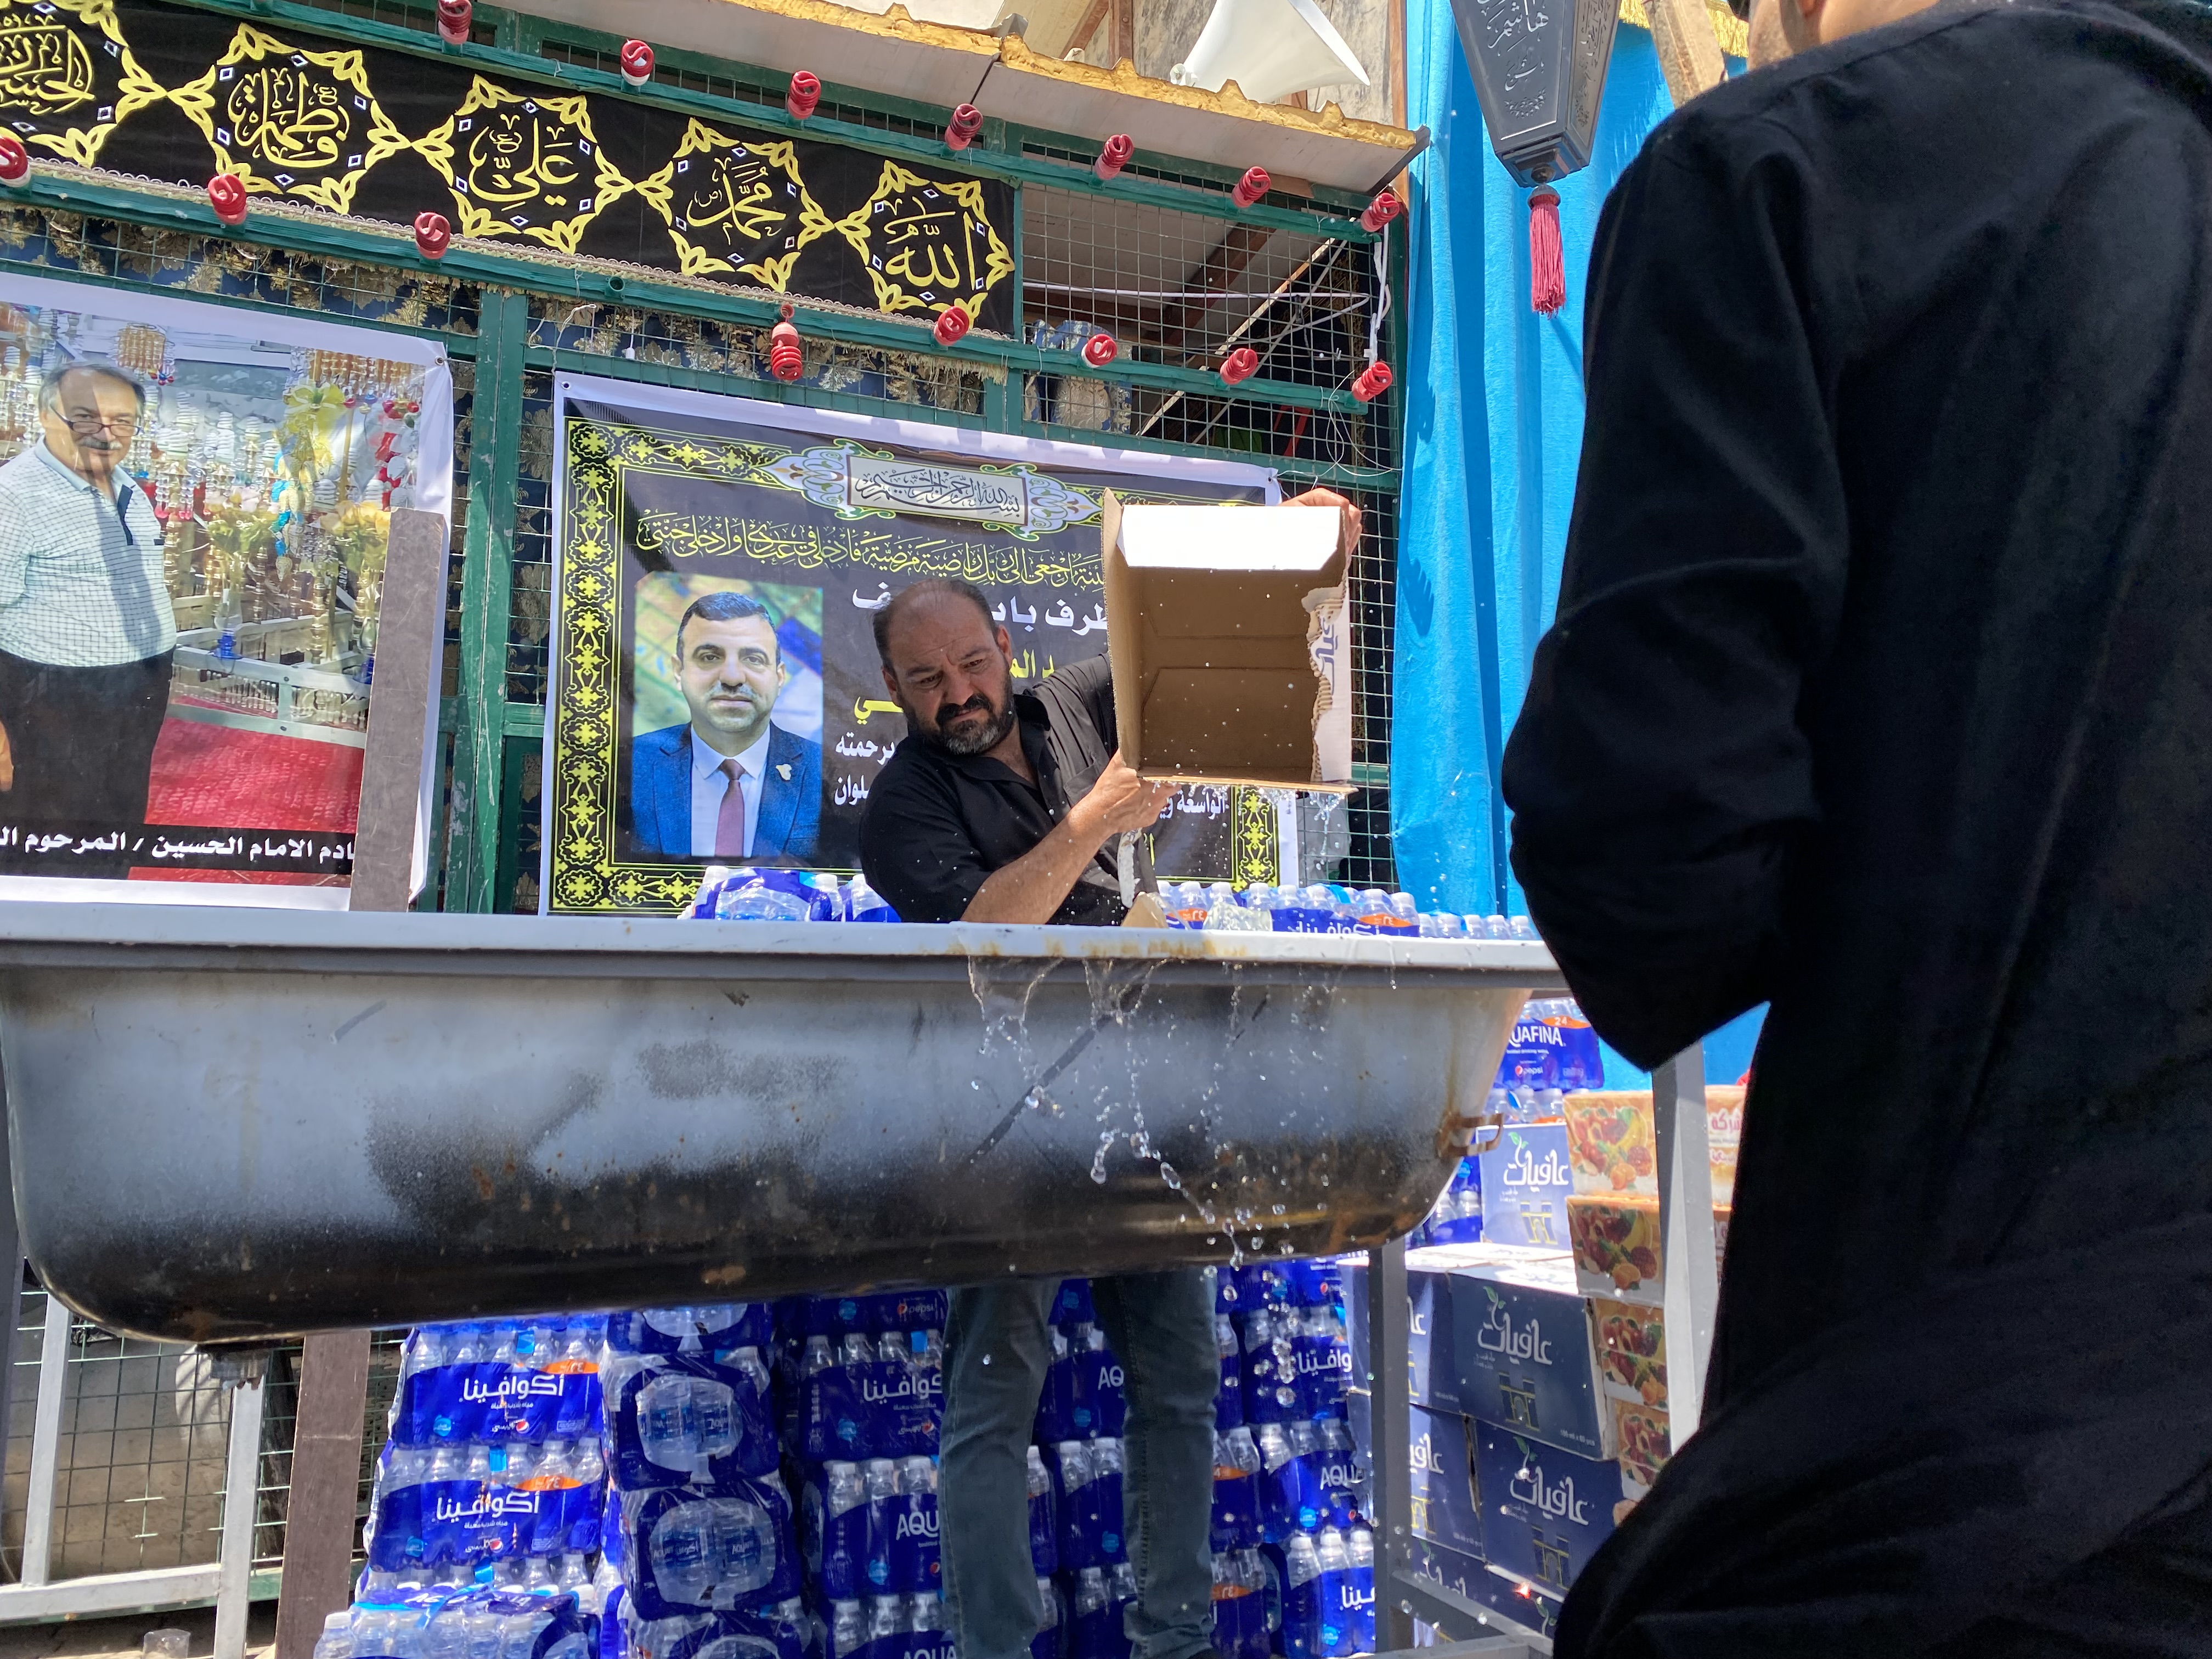
\includegraphics[width=0.5\textwidth]{images/pouring-water.jpeg}
% \label{fig:water-mowkeb}
% \end{figure}

As we reach the Shrine of Imam Hussein, we stumble upon a group of soldiers performing a salute in front of the shrine (see figure \ref{fig:hashd-salute}). These men are from the Hashd al-Shaabi, or Popular Mobilization Forces, the umbrella organization of militias that arose after 2014 to combat ISIS which I describe in detail in section \ref{city-and-militias-section}. 

\begin{figure}
\caption{An unidentified brigade of the Hashd al-Shaabi salutes with their brigade flag at the Qibla Gate of the Shrine of Imam Hussein. Photo taken by the author in August 2022.}\centering
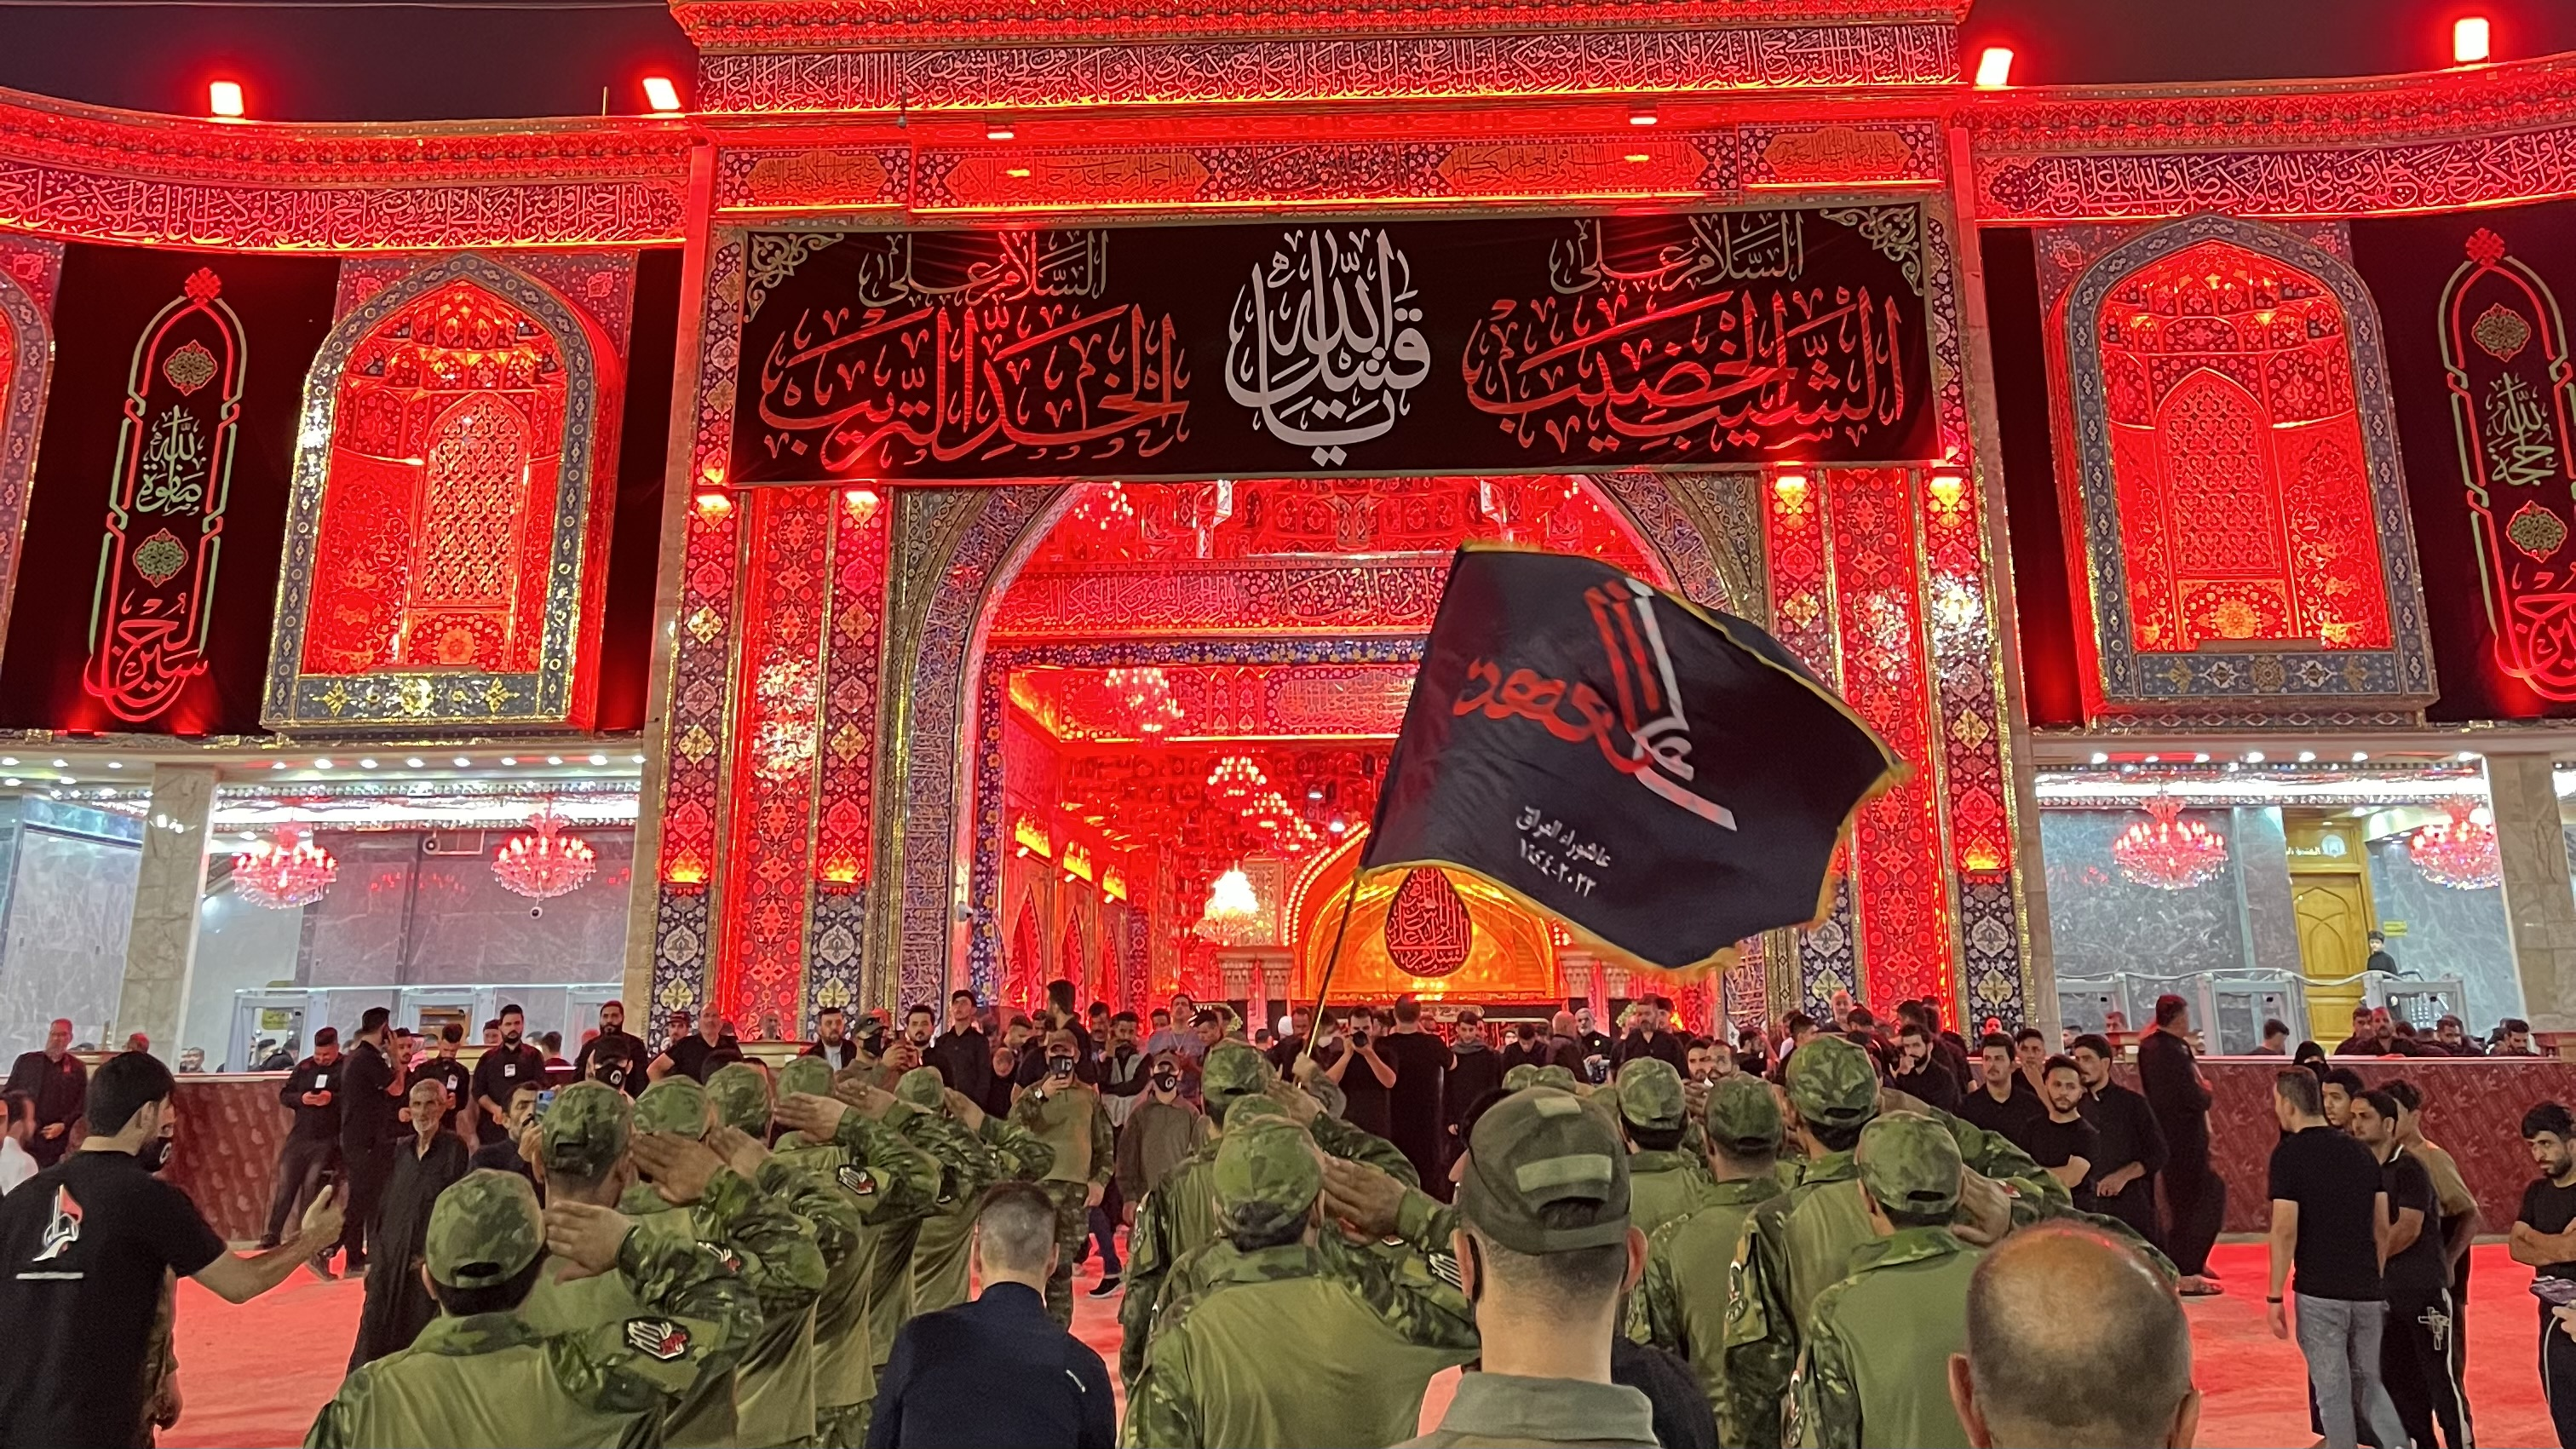
\includegraphics[width=.75\textwidth]{images/hashd-salutes.jpeg}
\label{fig:hashd-salute}
\end{figure}

Next to the soldiers, near the door of the shrine, I notice orators known as \emph{radūd}\footnote{Singular \emph{radūd}, plural \emph{rawadīd}} leading pilgrims in a ritual known as \emph{latm}\footnote{I describe \emph{latm} in detail in section \ref{latm-section}.}, a form of self beating where participants beat their chest to a liturgy, known as \emph{latmiya}\footnote{Singular \emph{latmiya}, plural \emph{latmiyyat}}. This ritual beating symbolizes the sacrifice and pain of Hussein. Billboards with the image of major clerics and their respective broadcasting channels loom behind us, while a \emph{mūkib} nearby blares a \emph{latmiya} called "Saleyt", or "Have you prayed yet?". 

% \begin{figure}
%   \captionsetup{width=.5\linewidth}
% \caption{Hashd martyrs displayed on the road to the Imam Hussein Shrine. Image taken by the author, August 2021.}
% \centering
% \includegraphics[width=0.5\textwidth]{images/hashd-martyrs.jpeg}
% \label{fig:hashd-marytrs}
% \end{figure}

This walk to the shrine is emblematic of the tension in the religious sphere in Karbala: the \emph{radūd} leading a ritual, the Hashd performing a military salute at the Qibla Gate of the shrine, and the clerical billboards looming above all. This chapter focuses on disentangling the various parts of this tension, focusing first on the the recent history of Karbala and the Hashd, then describing the role of the \emph{radūd} in rituals and how the \emph{rawadīd} have become a competing religious authority, trained through a parallel institution with the clerics. It ends with a description of two different majalis, a specific type of religious ritual which illuminates the differences of political power between the \emph{rawadīd} and the clerics. 

% I want to emphasize the burgenoning tension between the radoods, who are ritual orators 

% Among scholars of Iraq, Najaf's centrality and the so called "Najaf veto", which describes the role that Najaf plays in the central government has described and performs the authority. 

% While there exist multiple accounts of rituals between Ashura and Arbaeen, such as \emph{zangeel} (self-flagellation by chains), \emph{tatbir} (ritual cutting of the head), and \emph{latmiya} (self-beating often accompanied by elegies), there is significantly less focus on the institutions and structures surrounding \emph{husseiniyya} rituals. 

% Within anthropology, most pilgrimage studies have emphasized the temporary aspect of pilgrimage, treating it as a break from the pilgrim's routine. To date, the only known contemporary study of pilgrimage that attempts to approach pilgrimage as a permanent state of being is focused on the Shikoku pilgrimage, in which pilgrims often walk tens, if not hundreds of times within their lifetime \cite[9]{reader_pilgrims_2021}. While Reader and Shultz provide convincing arguments for understanding pilgrims, little focus is given to the people who provide for the pilgrims: the temples, bureaucracy, and culture surrounding it.

% - institutions matter, people aren't just touring
% - everything has agloomed onto the religious level, which actually is eating away at clerical authority 
%     - things that look like acts of faith don't automatically imply the growth of clerical power


% I want to emphasize the work institutions surrounding pilgrimage accomplish, and how pilgrimage has become a multifaceted site of contestation. While pilgrims and other pious subjects experience a market in the consumption and decision of spiritual authenticity \cite{moufahim_pilgrimage_2018}\cite{mujtaba_husein_phenomenological_2018}, the mechanisms which support these spiritual markets require constant labor and upkeep. Specific in Shi'ism within Karbala, the post-2003 environment has lead to a massive expansion of shrine institutions, which has caused previously clear authority lines to become muddled through increasing bureaucratization. Combined with the role the laity play in the Shi'a ritual of Majlis al-ʿaza contribute to making the majalis an environment where religious authority is constantly being negotiated. 

\section{The City and the Militias} \label{city-and-militias-section}
The oral history of Karbala suggests that it quickly became a pilgrimage site after the death of Imam Hussein, with tribes eventually settling in the area. This history is apparent from the way this city is structured, with the old city the urban topology deviates from the conventional pattern found in most cities, where the old city typically lies at the center. Instead, the old city of Karbala occupies a distinct section of the town, reflecting a unique spatial organization that has developed over time\footnote{See \ref{seven-great-mokwebs} for a more detailed description.}. 

The city has largely developed in an oblong shape, with the old pilgrimage sites jutting out from the middle. The old section of Karbala is only the shrine and surrounding areas. This status has led to a continuous influx of pilgrims and visitors, prompting the need to maintain the area's historical and religious integrity. Consequently, urban expansion has been focused on the areas surrounding the old city, ensuring the preservation of its unique character and heritage.

The shrines themselves have functioned as autonomous administrations for many areas of Karbala. Leaning into the explosion of post-2003 Shi'a \emph{awqāf} \cite{hamdan_development_2012}, the managerial institutions of the shrines known as the \emph{ʿatabat}  have developed many tentacles, becoming massive landholders in their own right. While \emph{awqāf} have largely disappeared across the Sunni Arab world \cite{moumtaz_gods_2021}, the \emph{ʿatabat}  have become massive landholdings and public work institutions, holding offices for public health, journalism, public relations, and so on. 

However, it is important to note that not only is Iraq within the post-2003 era, it is still dealing with the aftershocks of ISIS. The rise of the Hashd al-Shaabi following Ayatollah Sistani's engagement in the formation of the 2005 constitution \cite{al-rahim_sistani_2005} the 2014 fatwa \cite{rudolf_battlefield_2018}\cite{ann_wainscott_engaging_2019} have created a complex entanglement with the state in Baghdad, the poles of power in Najaf, and the variegated \emph{ʿatabat}. The creation of the Hashd al-Shaabi has entered a strange territory with respect to literal power. While the Iraqi army is locked behind of the aegis of the state and sources its funding from the state, the Hashd are described as a "hybrid-security actor", as they functions similarly to a gendarme but with little government oversight, drawing funding from both the state, Iran, and outside donations.\cite{cambanis_hybrid_2019} \cite{renad_mansour_popular_2018}. In addition, multiple Hashd groups and non-Hashd militias such as Sayara Salaam have control over entire cities: the city of Tel Afar, a Shi'a enclave in the Sunni province of Anbar, is completely run by members of the local Hashd division, including its police force and local government. The city of Samarra, near the shrine of Imam Askari, is run by Sayara Salaam, who exerts control over city council and checkpoints into and out of the city, extracting taxes and bribes over goods in transit. It is not uncommon to see a story or talk to militia members who confiscate material such as alcohol or electronics from truck drivers. 

Omar Sirri has written about how the network of checkpoints and the privileged access provided to the militias in Baghdad have dramatically changed the landscape, stating that "residents frequently noted how parastatal groups were ‘in control’ (msaitreen) of the city’s different districts" \cite[14]{omar_sirri_destructive_2021}. A similar process has been undertaken in Karbala, where militia symbols and logos adorn mosques and shops. 

Any visitor to Karbala will come across the Safeer Imam al-Hussein Surgical hospital next to the shrine of Imam Hussein. This hospital is funded and affiliated with the shrine itself, providing medical care for pilgrims during pilgrimage season, as well as general public health initiatives. The Safeer hospital is repeatedly shown in social media, photographers working for the shrine of Imam Hussein repeatedly show up to take photos, which are then published on the Imam Hussein website, available in over 6 languages, including Hausa. The Hussein shrine also has a research center dedicated to Shi'a history, publishing books and conducting archival work. The current manager of the Shrine of Imam Hussein is Doctor Nofour Abbas, who completed a masters in business management before taking up his role \cite{nofour_abbas_interview_2021}. Abbas mentioned that the \emph{ʿataba} participated in financing the Hashd after 2014, as well as providing funerals for deceased members. By his count, over 18,000 people work across various shrine institutions within all of Iraq. 

Interestingly, Dr. Abbas is from a sayyid family, meaning that he traces his lineage back to the Prophet. However, Dr. Abbas is not a cleric, he has never studied at a seminary in Najaf, and studied for his masters overseas. When I asked Dr. Abbas if the holy shrines were ever run by clerics following 2003, he mentioned that his predecessor was not a cleric. 

In competition with the Shrine of Imam Hussein is the Shrine of al-Abbas, whose \emph{ʿataba} goes by the name of al-Kafeel foundation. The al-Kafeel foundation is locked into an institutional rivalry with the shrine of Imam Hussein, they both host separate research centers for Shi'ism, parallel media arms, and extol the public for donations. 

Notably, al-Kafeel is responsible for the issuing of licenses for \emph{muwālkib}, which are tents that offer various services to pilgrims. Serving pilgrims is seen as a religious duty, and many Karbalaeis set up \emph{muwālkib} during the pilgrimage path, providing food, water, foot massages, and places to sleep and conduct religious rituals. However, due to the limited space within the old city of Karbala, bureaucratic control reasserts itself in order to manage the physical space. 

The bureaucratization of the shrines have opened up avenues of engagements for non-clerics in positions of power following 2003. Interviews with clerics and regular workers alike all suggested that no one questioned someone with business training instead of religious training; a few workers regarded this as a point of pride, noting that Dr. Abbas was a very serious man. 

% It is unclear how the various bureaucratic spheres were carved out between the two shrines. While al-Kafeel manages the \emph{muwālkib} licenses, the shrine of Imam Hussein has taken the role of public works projects for various groups, such as the women's hospital and autism research center. When I asked the manager of the Department of Muwalkib how the current bureaucratic state came to be, he shrugged his shoulders and answered, "we got they permission from the government, the \emph{ʿataba} didn't", and guided the conversation to a different topic.

\section{\emph{Husseiniyya}}
A \emph{husseiniyya}\footnote{Singular \emph{husseiniyya}, plural \emph{husseiniyyat}} (not to be confused with the adjective used in \emph{shʿir husseiniyya}) is a mix between a mosque and a community center. All mosques within Karbala and all Shi'a mosques across southern Iraq are \emph{husseiniyyat}. Beyond acting as sites of worship, \emph{husseiniyyat} host various community events, such as Qurʾan classes and liturgy classes, and act as rest stops for pilgrims.

Within Karbala, many \emph{husseiniyyat} are endowed by specific wealthy families or have particular political affiliations. Large photos of these patrons are hung inside the \emph{husseiniyya} itself. For example, Husseiniyya Shirazi is ideologically affiliated with Ayatollah Sadiq al-Shirazi from Iran and displays a backlit picture of al-Shirazi on top of the entrance and prominently on the back wall of the \emph{husseiniyya}. Husseiniyya Khadimat Ahlu Bayt similarly has two photos of the two patriarchs of the patron families of the \emph{husseiniyya}.

A \emph{husseiniyya} also collects donations from its attendees, often to serve pilgrims. A friend in Najaf mentioned that her family "gives everything to the \emph{husseiniyya}, including old furniture and spare cash." This is in addition to the \emph{waqf} endowment, and on top of the Shia \emph{khums}, a one fifth tithe on certain sources of income that many Shi'a Iraqis pay to the organization of Ayatollah Sistani.

\section{Majlis al-Hussein and Majlis al-ʿaza}
There are two main types of Shi'a majlis: Majlis al-Hussein and Majlis al-ʿaza. Both share specific features, but the key distinction is that Majlis al-ʿaza is accompanied by a \emph{latm} at the end, whereas Majlis al-Hussein is not.

The distinction arises from the purposes of the majalis: Majlis al-Hussein is intended to be a "happy majlis of celebration," \cite{al-husseini_interview_2022} whereas Majlis al-ʿaza is meant to be a ritual of mourning. The liturgical nature of \emph{latm} makes it appropriate only for the Majlis al-ʿaza.

Both majlis begin with a sermon called a \emph{niyaha}\footnote{Singular \emph{niyaha}, plural \emph{niyahat}.} and delivered by a religious leader, usually a tribal sheikh or someone from the \emph{ulama} \cite{hamdan_development_2012}, although another religious leader from the community may be selected. Multiple discussions with \emph{rawadīd} implied that the sermon giver required little more than acknowledgement from the local community, many \emph{rawadīd} double as sermon givers, such as the case of the \emph{radūd} in Husseiniyya Shirazi, described later. The sermon may be on any topic, although they are typically focused on a specific story relating to Hussein. For Majlis al-ʿaza, this may be a specific story relating to sacrifice or tragedy during the Battle of Karbala, while for Majlis al-Hussein, the sermon may focus on themes such as an Imam's birth and related celebrations.

After the sermon, both majlis will bring a liturgical reciter, known as a \emph{radūd}, up to the stage. For Majlis al-Hussein, the \emph{radūd} will perform a "happy" song, in which the audience will either clap or chant along. For Majlis al-ʿaza, the \emph{radūd} will perform a liturgy known as a \emph{qaṣīda}\footnote{Singular \emph{qaṣīda}, plural \emph{qaṣā’id}}, and the audience will engage in chest-beating in accompaniment, known as \emph{latm}. The entire ceremony is called a \emph{latmiya}. During my fieldwork in Husseiniyya Khadmiat al-Bayt, a \emph{husseiniyya} with donations from multiple notable families within Karbala, many ritual participants would arrive towards the end of the \emph{niyaha} or the beginning of the \emph{latmiya}.

Notably, the sermons in Karbala are conducted in Iraqi Arabic and not Modern Standard Arabic (MSA). Throughout my fieldwork in Karbala, I did not find a single Shi'a ritual conducted in MSA. This distinction is notable because Khutba, the equivalent of a Friday sermon for Sunnis, is always conducted in MSA. This distinction may arise because the Shi'a, as the religious minority within Islam, may feel it is necessary to be as inclusive as possible, as many Iraqis do not completely understand MSA. This method of inclusion mirrors how Shi'as often proclaim cross-sectarian affiliations not necessarily as an inherent tolerance but as a function of demographics, as suggested by Fanar Haddad\cite[183]{haddad_understanding_2020}. Several of my Sunni interviewees from Baghdad remarked with disdain when I mentioned that the Shi'a conducted their rituals in colloquial Iraqi Arabic, with one referring to how "they [the Shi'a] do this because they have no culture." During an interview with Muntazir al-Husseini, a \emph{radūd} affiliated with the the Karbala Center for Studies and Research, he mentioned that the entire Majlis is conducted in colloquial Arabic because it would be confusing for one to switch between MSA for the sermon section, only to transition to colloquial for liturgy. This distinction seems to highlight the differences between an "us" and "them", especially in such a charged sectarian environment in the post-ISIS years. 

\section{\emph{Rawadīd}} \label{radood-section}
A liturgical performer, known as a \emph{radūd}, typically leads the audience in a \emph{latmiya}. The \emph{radūd} is responsible for selecting the appropriate chant and guiding the audience. As an active participant in the recitation, the \emph{radūd} often moves to the beat and provides prompts for the audience to chant or move.

During my fieldwork, I attended multiple sessions at the \emph{radūd} school located in Husseiniyya Yassine on Mohammad Yamine Street. Friday sessions are divided between Qurʾan classes in the morning and \emph{radūd} practice in the afternoon. While Qurʾan classes are conducted in formal Arabic, the \emph{qaṣā’id} performed by the \emph{radūd} are in Iraqi Arabic, with Friday classes providing Qurʾan instruction in the morning and \emph{radūd} practice in the evening.

\emph{Radūd} classes are structured similarly to voice lessons, as students receive instruction on which parts of the mouth produce specific sounds and when to breathe during performances. Following the initial vocal training, students are expected to take the stage and perform a \emph{qaṣīda}, while their peers and the teacher provide guidance. This process is repeated for each student, who can come from any background or neighborhood and is not required to belong to a prominent family. Though multiple schools exist within Karbala, Husseiniyya Yassine is considered the most notable one, with several interviewees praising the skills of the teachers.

The teacher for the Husseiniyya Yassine school is a man named Ali, who typically works at the municipal water ministry. Like the other teachers, he was once a \emph{radūd} himself, but now volunteers his time at the \emph{husseiniyya}, training younger generations. Similarly, there are specific \emph{rawadīd} for the Hashd groups, although anyone is welcome to see their performances. 

A poet provides the poems that the \emph{radūd} performs. While \emph{rawadīd} sometimes perform their own poems, many poets often vie for the opportunity to have their poetry performed by a \emph{radūd}. As \emph{muwālkib} are usually associated with a specific house or neighborhood, they typically have only a single \emph{radūd}, who might be invited to perform or originate from that particular area. However, for a single \emph{mūkib}, there may be multiple poets, who similarly can come from any region. 

A possibly apocryphal story about one of the most famous \emph{radūd}, Bassam Karbalei, claims that he receives poems at night from various poets and proceeds to perform them without practice the next day as a display of his skill\cite{al-husseini_interview_2022}. Individual \emph{rawadīd} still hold great sway; Karbalei's predecessor, Hamza al-Zghayer, continues to resonate with many Karbaleis. 

\emph{Rawadīd} have a far more diverse background than clerics. While the most famous clerics are typically descended from sayyid families, \emph{rawadīd} can come from any neighborhood, and do not have titles. Clerics must attend seminaries such as the famous \emph{hawza} in Najaf in order to reach various ranks, but anyone is eligible to be a \emph{radūd} \cite{al-husseini_interview_2022}. During my fieldwork, the school at Husseiniyya Yassine was graduating a blind \emph{radūd}. A \emph{radūd} joked that "there were more \emph{rawadīd} than attendees," referring to the substantial increase in the number of \emph{rawadīd} since 2003. The same interviewee mentioned that many members of the 'ulema found this rise uncomfortable, as people tend to believe what \emph{rawadīd} say instead of what the 'ulema say \cite{al-husseini_interview_2022}. Compounding this issue is the fact that while \emph{Hawza} is a religious institution where classic and MSA are venerated, \emph{radūd} training is conducted entirely in Iraqi Arabic. 

\emph{Rawadīd} often travel to perform in other Shi'a majority countries as well, such as Bahrain and Lebanon. The same interviewee noted that when he performed in Lebanon and Bahrain, many of his colloquial phrases were not understood, as he relied too heavily on Iraqi expressions.

\section{\emph{Latm} and \emph{Latmiya}} \label{latm-section}

A \emph{latm} (literally "slap") is a form of self-beating, often on the head or chest. Those who perform \emph{latm} typically do so in response to a sermon or a \emph{latmiya}, viewing the pain as a means to become closer to the sacrifice or pain experienced by Imam Hussein.

\emph{Latm} can be performed in various ways, with or without a specific reciter. There are few rules dictating where a \emph{latm} can take place. From my experiences, any religious site with available space during pilgrimage season might be occupied by young men performing \emph{latm}. During the visitation to Kadhimiya, I witnessed \emph{latmiyyat} being performed in the street by young men who were listening to a \emph{latmiya} played on a mobile speaker. Around the shrines in Karbala, any open space was likely to be taken over by \emph{latm} participants.

\emph{Latm} groups around the shrines were often organized along national, tribal, or neighborhood lines. The Iraqis living in Karbala shared various stereotypes about the groups who performed \emph{latm}: Pakistani \emph{latm} participants were perceived as very violent, while Iranian \emph{latm} participants were considered to have a quicker rhythm. These national lines are complemented by differences along tribal and neighborhood lines, tribal Arabs from south Iraq will perform a \emph{latm} alongside a ritual known as \emph{hosa}, a tribal ritual where men rhythmically stomp and spin in a circular motion while chanting lines of poetry, while \emph{rawadīd} of specific neighborhoods pick different \emph{qaṣā’id} to align with the political affiliation of their neighborhood \footnote{See section \ref{seven-great-mokwebs} for a description of neighborhood differences in Karbala}. 

In these spontaneous \emph{latm}, participants would arrange themselves facing each other, sometimes in a circle but often haphazardly. Sometimes a \emph{latmiya} would be played on nearby speakers, but at other times, the participants would chant the \emph{latmiya} themselves while beating their chests.

While spontaneous \emph{latm} is common, a \emph{latmiya} with a \emph{radūd} typically requires more organization, specifically space for participants and speakers. The numerous \emph{husseiniyyat} and \emph{muwālkib} provide this space, often including complex sound systems and large speakers. I spoke with an electronics shop owner in Karbala at a cafe who mentioned that the majority of his business came from buying and selling speakers for various \emph{muwālkib} and \emph{husseiniyyat} during pilgrimage season.

For \emph{latmiyyat} involving \emph{rawadīd}, participants can either arrange themselves in rows facing the \emph{radūd} or facing each other in circles. I noticed that during \emph{radūd} \emph{latmiyyat}, men would take their shirts off, which I attribute to the fact that \emph{radūd} \emph{latmiyyat} are typically performed in a more private, confined space, whereas spontaneous \emph{latmiyyat} in the streets are more public.

One of the key distinctions of \emph{latm} and \emph{latmiya} is its inclusive nature. During my fieldwork, I was struck by how often \emph{rawadīd} would engage their audience by encouraging them to participate in the chant, often accompanied by shouts of "yallah shabab!" (a phrase used to encourage the audience). \emph{Rawadīd} would leave space within their qasa'id for audience members to chant the refrain after the \emph{radūd} had repeated it several times. Often, but not always, audience members would remove their shirts and arrange themselves into circles facing each other rather than the \emph{radūd}.

The symbolism here is striking: a religious ritual performed in the local vernacular, with audience members participating and facing one another instead of the orator. The ritual is set up in an inclusive and egalitarian manner; while the \emph{radūd} leads, audience members are expected and encouraged to chant the same lyrics alongside the \emph{radūd}. The use of Iraqi Arabic instead of MSA emphasizes its inclusivity among Iraqis, reinforcing notions of authenticity. As Fanar Haddad mentions "Shi'ism needs the validation of Sunni acceptance in order to survive as a recognized part of mainstream global Islam; needless to say, the reverse does not hold" \cite[179]{haddad_understanding_2020}. The minority role of Shi'ism creates a politics of inclusion: while Sunni sermons may be free to exclude audiences in the usage of MSA, the Shi'as must cast as wide of a net as possible, turning themselves to the local vernacular\footnote{It is also interesting that many Shi'a \emph{qaṣā’id} within other countries use the local vernacular: \emph{rawadīd} in Lebanon use Levantine Arabic, \emph{rawadīd} in Pakistan use Urdu, and British \emph{rawadīd} use English. In Karbala, a common site is seeing one group of pilgrims participating in a \emph{latmiya} in Urdu next to another group using \emph{Azeri}. 
% This mirrors the effect of the Vatican II accords where the Vatican council declared that liturgies must be performed in the local vernacular instead of Latin.
}. The arrangement of audience members into circles facing each other further emphasizes that the ritual is not meant to reinforce the position of the \emph{radūd} but rather to connect the audience to each other and their belief in the pain of martyrdom and sacrifice.

\section{Majlis} \label{majlis}
Majalis are diverse and politically charged events. The term "majlis" is used in the Karbalaei context for any religious gathering involving a \emph{radūd} and/or a religious elder. They consistently follow the same format: a sermon known as a \emph{niyaha} at the beginning, typically delivered by a religiously educated person such as a sheikh, though not necessarily ordained. This is followed by a performance by a \emph{radūd}. While some majalis may omit the \emph{radūd}'s performance, sermons cover a wide range of topics and are always conducted in Iraqi Arabic.

Attending a majlis is a deeply intimate experience. Upon entering, one is immediately struck by the ornate decorations, which include calligraphic designs, intricate poles, and often images of marja'. More elaborate majlis locations are promoted in advance on social media, with renowned \emph{rawadīd} drawing attendees from across Iraq. A majlis with Bassam Karbalaei will typically overcrowd the shrine, leading the shrine attendees to ban women from the shrine courtyard. Individual \emph{rawadīd} also advertise their upcoming appearances on platforms like Instagram and Telegram, using their channels to share details about their next performances.

Before attending a majlis, participants are usually treated to tea and socialization, with people frequently gathering outside the venue. Specific venues are associated with particular \emph{husseiniyyat}, which are, in turn, linked to neighborhoods or families. Khadamat Ahlu Bayt and Khadamat Ali al-Akbar are two \emph{husseiniyyat} that host larger majalis between Ashura and Arbaeen, while various \emph{muwālkib} host impromptu majalis throughout the city. Attendance at majalis peaks during Arbaeen and the night before, as pilgrims arrive from different cities in Iraq. While Ashura pilgrims are predominantly Iraqi, the week leading up to Arbaeen sees an influx of foreign pilgrims in Karbala.

\emph{Radūd} performances have few rules. Although some \emph{rawadīd} may have received vocal training within a school, many have not. \emph{Rawadīd} are often chosen at a young age for their vocal talent and intonation. Being a \emph{radūd} is seldom a full-time job; all the \emph{rawadīd} I encountered held other jobs, such as waiting tables in Baghdad, working at the Shrine of Imam Hussein, or holding government positions. When asked about their motivation, they described the pursuit of becoming a \emph{radūd} as a passion, rather than a specific goal.

\subsection{Husseiniyya Shirazi}
One of the more unusual \emph{radūd} performances I attended took place at Husseiniyya Shirazi, where locals often referred to the \emph{radūd} and participants as "crazy." This small \emph{husseiniyya} is located off the road leading to the Qibla gate in the Shrine of Imam Hussein and is notably drenched in red. Even before entering, the reverberations and echoes of the \emph{radūd} are audible from the street. Concealed behind a few stalls, a photo of Grand Ayatollah Sadiq Shirazi is displayed on the awning outside the \emph{husseiniyya}. The reputation of this \emph{husseiniyya} is well known; a female journalist friend who came to Karbala was warned against going there, as if the local Karbalaeis found it shameful for a woman to attend. The overwhelming majority of participants were local, and all young males. However, as a man, I had not been cautioned against this place beforehand.

Upon entering, it was immediately apparent that the atmosphere was entirely different from other \emph{husseiniyyat}. The \emph{radūd} performance varied significantly, with a heavy use of echo and chanting that bordered on screaming. Deep-throated chants of "Hussein Hussein" were prevalent throughout the entire performance, accompanied by lighting reminiscent of a heavy metal concert. Dark crimson enveloped the room, with only a brightly lit photo of Ayatollah Shirazi in blue standing out among the sea of red. The room itself was also quite small, nearly half the size of typical \emph{husseiniyyat}, although this might have been due to size restrictions on buildings near the shrine.

Rhythmic beating, which is often optional in performances, played a prominent role here, with loud drums resonating through the speakers. A single microphone hung in the middle of the room, connected to speakers to provide significant reverberation.

\begin{figure}
\caption{A typical majlis at Husseiniyya Shirazi. Men take off their shirts and perform a \emph{latm} while the \emph{radūd} keeps the beat. Image taken by the author, August 2022.}
\centering
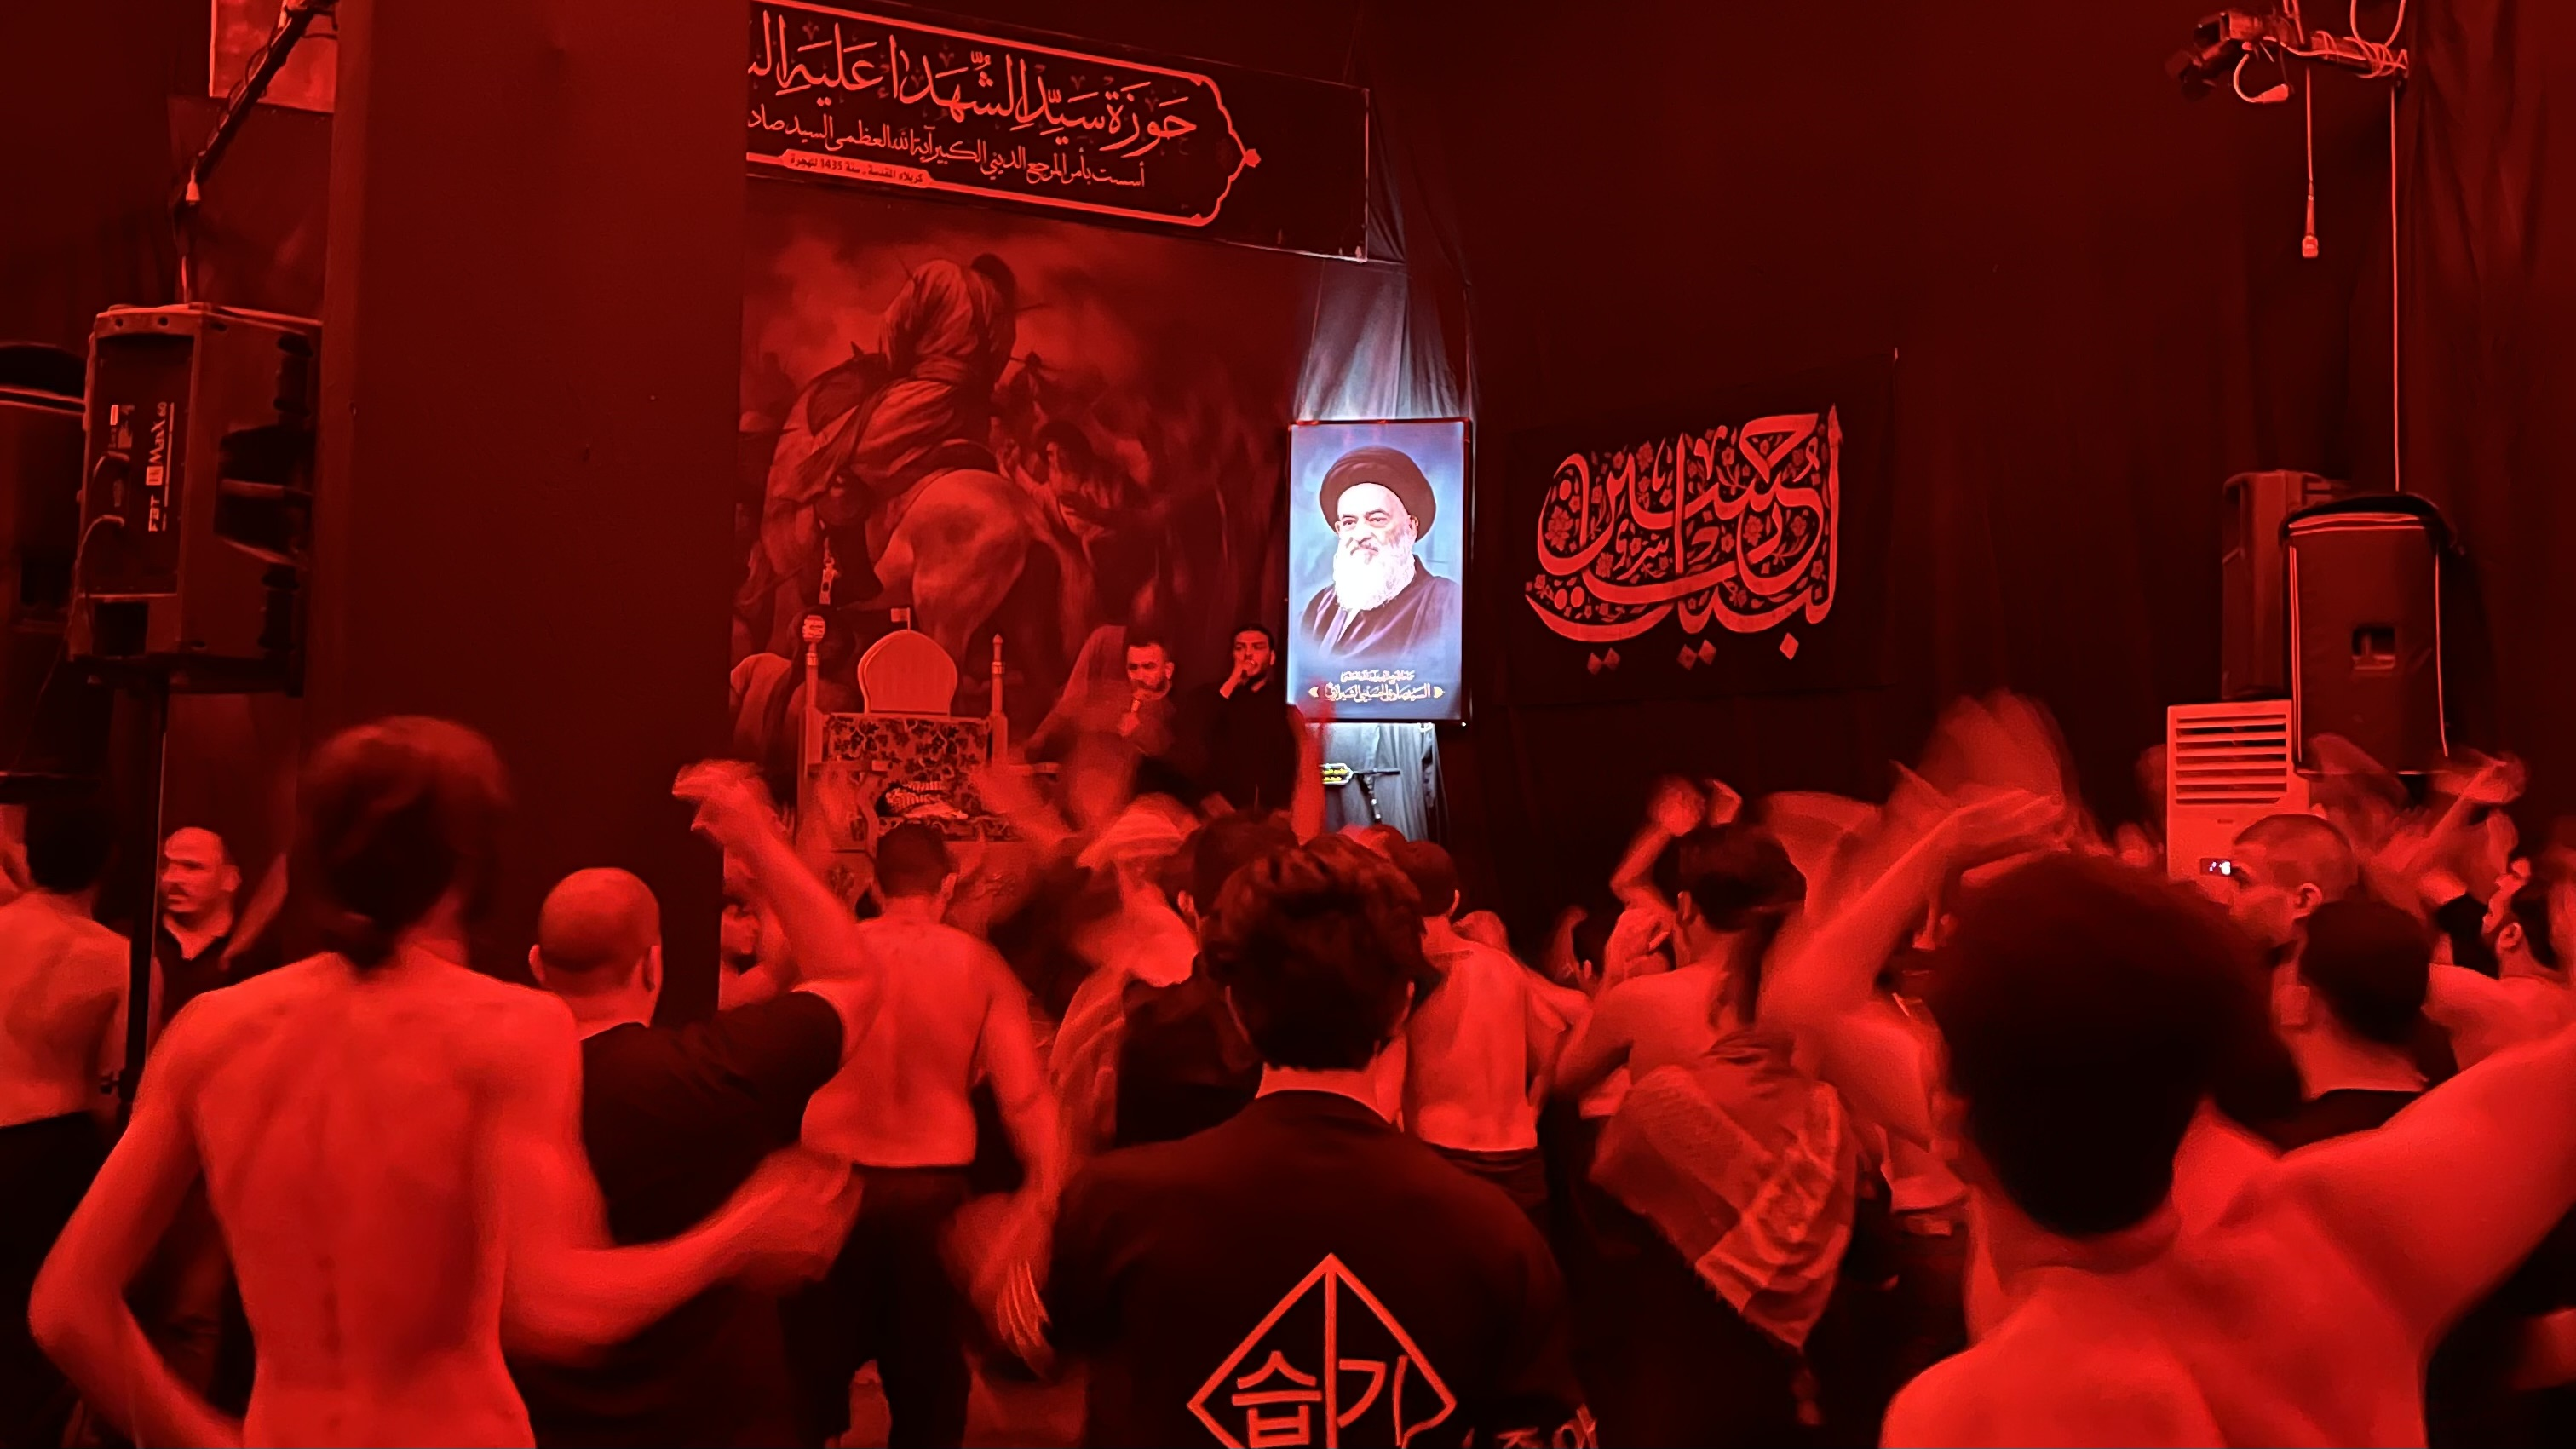
\includegraphics[width=.75\textwidth]{images/shirazi.jpeg}
\label{fig:shirazi}
\end{figure}

Instead of forming circles, as is common, people positioned themselves around the \emph{radūd}. As expected, the attendees were exclusively shirtless young males, beating themselves in rhythm with a booming beat, giving the performance a rave-like atmosphere (see Figure \ref{fig:shirazi}). The same \emph{radūd}, a man in his mid-30s with a rugged beard, performed both \emph{niyaha} and \emph{qaṣīda} each time. However, he declined to be interviewed by me.

Husseiniyya Shirazi continued to be a recurring fieldwork site for me, both due to its close proximity to the shrine and its uniqueness compared to other \emph{husseiniyyat}. I often observed young males gathered outside the entrance, hesitantly peeking their heads in as if afraid to enter. During another performance I attended, I witnessed a young man so overcome with grief for Hussein that he repeatedly attempted to grab the \emph{radūd}. Sobbing uncontrollably as if possessed, the \emph{radūd} had to push him aside to continue the performance. The lack of reaction from the rest of the audience was surprising, it seemed to imply that this was a common occurrence. This young man continued to double over in grief throughout the entire majlis, screaming and crying out "Hussein!" When the majlis ended, I approached and spoke with the young man, who casually explained that he was simply "overflowing with sadness." His friends informed me that the young man was from Hayy Abbas, a lower-income neighborhood to the north of the shrines.

I interviewed a different young man named Ali from Samarra, who mentioned that he had attended the Husseiniyya Shirazi rituals for multiple years. When asked about the changes between the years he had been attending, Ali mentioned that "the rituals have become more rhythmic, and involve more beating. We have a strong community, people like me\footnote{Referring to participants from Samarra.} and Basrawis come to this ritual. People who stay for a few times [to Husseiniyya Shirazi] stay forever here." Ali went on to describe how he had gone to many different \emph{husseiniyyat} to rituals before, but none of the \emph{rawadīd} had interested him until his friend brought him to Husseiniyya Shirazi the first time in 2017. He has been an avid participant, raising money for the husseiniyya every year. 

Locals describing participants as crazy is reminiscent of criticisms directed at repeat pilgrims on the Shikoku pilgrimage, where pilgrims seek to undertake the pilgrimage again after completing it once. In the case of the Shikoku pilgrimage, people living along the pilgrimage route have suggested that "compulsive pilgrims are simply substituting one addiction for another" \cite{reader_pilgrims_2021}. Similarly, Salafis who obsess over ablutions have been labeled as "neurotic" by observers \cite[67]{gauvain_salafi_2013}.

What one outgroup perceives as a "substitution of addiction" or  "neurotic" is regarded as a common activity by the ingroup. All these activities, while displaying a striking outward appearance, are carried out in a nonchalant and calm manner. Even though the young man was overcome with grief, the participant quickly regained his composure afterwards. Whether it be pilgrims in Shikoku who are seen as addicts pursuing a behavior, Salafis who are seen as having an unhealthy attachment to purity, or Shirazi participants whose screams and chants are viewed as crazy, repetitive ritual acts that alienate others serve to create a tighter ingroup. This, in turn, fosters a space for ritual evolution, pushing and engaging the boundaries of what tradition permits.

Although Husseiniyya Shirazi had both political and visible differences compared to the rest of the majlises, photographs continued to play a central role. During each performance, at least two or three phones were actively recording throughout, often with someone clearly livestreaming it on Instagram.

\subsection{Husseiniyya Qazwini}
The al-Qazwini family originally hailed from Iran, settling in Karbala during the late 18th century. In contrast to the Shirazi majlises, the Qazwini majlises were more standardized. A male member of the Qazwini family usually delivered a lecture at the podium, often reciting a story related to Hussein. I attended two different majlises, one before Ashura and another after. On both occasions, the \emph{niyaha} consisted of a similar story about the sacrifice of Hussein, citing specific tales of redemption and sacrifice. For instance, the majlis performed by Ali Qazwini before Ashura focused on the concept of supplication:

% \begin{quote}
% \begin{Arabic}
% شنو ليلة العاشر الحسين يكول "القوم لا يريدون غيري, لا يطلبون الا دمي, اذا ضفرو بي ذهلو عن غيري, اتركوني وعيالي." شوف شيصير, ذاك يكوملة شيكلة "لو متت ثم احييت" هذا يكوملة يكلة "ثم احرقت" ذاك يكلة "لو نُسفت" هذا يكلة "لو جعل بي كذا ما تركتك." هذا يكلة كذا هذاك يكلة كذا, ولهذا خلو الحسين يكول كلمة المعروفة المشهورة المحفوظة "لا اعلم اصحاباً" مو رأيت "لا اعلم" هواية فرق, ما ادري الاخوة يفرقون بين الاثنين لو ميفرقون؟
% \end{Arabic}
% \end{quote}

\begin{quote}
On the tenth night, Hussein says "The folk only want me, and they ask only for my blood, and if they succeed [in my death], they do not want to ask for anyone else, leave me and my children. See what shall happen, someone rises and says "if I died and was resurrected" and another says "then I was burned", another also rises and states "if I was blown up", and another says "even if something happens, I shall not leave you." This one declares and another declares. That is why they made Hussein say his well-known, well-quoted words of "I do not know of companions", he did not respond "I do not know", a big difference. Do you [all] know the difference between the two?
\end{quote}

I have reproduced this line in its entirety, as it exemplifies the typical majlis. A familiar story is narrated to an informed audience, and a brief exegesis is performed on the story to extract a specific moral. The audience is arranged in such a way that generally upper-class individuals, such as sayyids, celebrities, and prominent figures, are seated next to the reciter, while the commoners are positioned further back. Due to the room's layout, chairs along the way are generally reserved for members of the Sayyid family. I observed multiple instances where people would vacate their chairs and offer them to a Sayid or cleric who had just entered the room.

Similar to the Shirazi majlis, the audience is expected to fulfill a specific role in lamentation. During the \emph{niyaha}, the audience follows along and occasionally chants blessings upon the Prophet and his family when prompted by the reciter. At other times, audience members are expected to cry and lament by placing their hands on their faces and weeping.

Towards the end of the Qazwini majlis, instead of a \emph{radūd} and \emph{latm}, the reciter performs a short recitation with a different intonation. Rather than using the white lights present throughout the rest of the room, a family member switches the lights to a blood-red color, creating a dramatic visual effect. Audience members cry out and weep, often repeatedly striking their own forehead, face, or chest, using pain as a means to bridge the temporal gap towards the imam.

All Qazwini majalis are livestreamed. A phone is placed near the reciter, using Instagram Live to stream to several thousand followers. Each member of the Qazwini family, particularly those based in the United States, carefully maintains a social media presence. Similar preachers have emerged across the Islamic world; Turkish clerics have attracted millions of views\footnote{See https://restofworld.org/2021/the-cleric-has-uploaded-a-new-video for an explanation on the rise within the Muslim workd.}, Saudi preacher Abdul Aziz al-Ansari and Egyptian preacher Dr. Haitham Talaat each have hundreds of thousands of followers on YouTube. Mid-level clerics in Iraq also boast comparable social media followings, competing with \emph{rawadīd} for attention. Heavily edited imagery, often featuring photoshopped chains or blood, frequently appears within Telegram channels.

Compared to Husseiniyya Shirazi, where the entire audience was completely composed of young men, where no one wore a turban, Husseiniyya Qazwini was filled with older men in a sea of black turbans. In an interview with Ali Qazwini, who is 21 years old, he mentioned that his family often puts him in charge of public events, as he is seen to be more relatable to most Iraqis. According to the United Nations Development Program in 2021 \cite{undp_youth_2021}, over half of the 40 million Iraqi are under 25, which exerts significant pressure on the clerical class. 

\section{Competition in the City and Religion}
Karbala's growth following 2003 has led to explosions of \emph{awqāf} and charities, but has also notably failed to achieve significant progress in infrastructure since 2003. Water from tap remains non-potable, electricity still relies on generator power to supplement government electricity, and public health care has largely declined. These lacunae have largely been filled by the shrines, such as the recent opening of the women's hospital affiliated in 2022 and the launch of Iraq's only autism center \cite{imam_hussain_holy_shrine_imam_2020}, both affiliated with the Shrine of Imam Hussein. The financing of the Hashd have made the \emph{ʿatabat} a central part of Iraqi life, the \emph{ʿatabat} tolerate Hashd symbols and provide them with space to place donation boxes. This has placed them in direct competition with the weak Iraqi state on the political level, the policies of the \emph{ʿatabat} matter far more to Karbalaei residents than the work of the central or municipal governments, with public works projects being funded through the various \emph{awqāf} that are funneled through the \emph{ʿatabat}. 

When I originally arrived in Karbala, I asked many of my interviewees about their choice of \emph{marjiʿ}\footnote{Singular \emph{marjiʿ}, plural \emph{marājiʿ}}. In Shi'ism, the \emph{marjiʿ} is a highest ranking senior cleric that a follower of Twelver Shi'ism chooses to emulate. I asked people about their choice of \emph{marjiʿ} expecting a process of rational deliberation, but the majority of my interviewees responded were befuddled with my question, and found it odd to ask at all. While all of them could name their \emph{marjiʿ}, in only two cases did any of them reply with a process that was rational deliberation, the majority of them responded that their choice in \emph{marjiʿ} was due to influences from their social circle or families. I had expected asking about \emph{marjiʿ} would lead to a clear explanation about sources of authority, only to find that the answers were rooted in community contexts.

In parallel to the political competition, a religious competition has also emerged. The \emph{rawadīd} occupy a unique role as they hold a position of religious authority while being outside the clerical class. \emph{Rawadīd} are often affiliated with the laity, using social media to draw audiences and speaking only in colloquial Arabic. When I interviewed a cleric who preached at the Shrine of Abbas, he complained that the "people listen to them [the \emph{rawadīd}] more than me now." Other clerics in informal discussions expressed similar thoughts, speaking to a shift in the ways Karbalaeis relate to their religion. 

This points to the two shifts of Karbala institutions in the post-2003 and post-ISIS environments: the merging of the clerical class into a state-like managerial class, and the loss of clerical influence to a rise in \emph{rawadīd}. Both of these have made Karbala an ideological battleground: pilgrims and residents are implored to donate to not just the shrines, but to various \emph{awqāf}, to the Hashd, to the \emph{rawadīd}, and to the \emph{husseiniyyat}. The rhetorical merging of initiatives onto the religious level has opened the floodgates to competition of pilgrim attention and donations. Pilgrims and residents are not simple consumers of religion, their acts and attendance in Karbala has political ramifications. Take the seemingly simple choice of choosing to attend majlis as Husseiniyya Shirazi or Husseiniyya Qazwini. Choosing Qazwini reinforces clerical authority, while choosing Shirazi reinforces \emph{radūd} authority. Another simple act of choosing which shrine to attend, whether the Shrine of Imam Hussein or the Shrine of Abbas, means supporting parallel bureaucracies. While it is obvious that each individual choice has an effect on the structures around it, the merging of all these facets onto the religious level and into the same ontological category of "Shi'ism" have made individual acts incredibly potent. 

As described in the beginning of the chapter, the area outside of Qibla gate is overflowing with meaning. The revival of \emph{rawadīd} after 2003 and the creation of the Hashd as a new form of authority after 2014 has begun to contest with clerical authority. The growth and formalization of \emph{radūd} schools, which bypass the traditional clerical route of \emph{hawza} has created an alternative source of religious knowledge and formed new religious identities for Karbalaeis to choose from. Clerics this as well, mid-level clerics now adopt similar imagery and social media tools like the \emph{rawadīd}. The Shi'a public sphere, which had dramatically expanded in size after 2003 due to the lifting of Saddam-era restrictions, was previously big enough for all players. Now the same sphere has become crowded.

However, this contestation of authority is not a new phenomenon. As we will see in the next chapter, the \emph{muwālkib}, one of Karbala's oldest institutions, is also responsible for ethical self-fashioning outside of the clerical class. 